\section{Analysis and Limitations}

\subsection{Residual Size Is Not Sufficient}

Residual magnitude is useful diagnostic information, but it is not a standalone safety predictor. R023 has low residual magnitude and high cosine to the frozen embedding, yet misses the COCO gate. R028 improves COCO under a similar small residual budget, while R029 has a larger residual and slightly lower COCO than R028. Anchor-20 runs reduce residual drift further, but do not solve COCO seed fragility. The direction and objective of the residual matter, not only its norm.

This point matters because residual methods are often described as safe by construction. RRB is safer than the hard replacement bottlenecks in this run history, but the residual form alone is not the safety argument. A residual can still move examples in directions that damage nearest-neighbor structure, which is also why preservation-oriented residual-gradient methods are relevant comparison points~\cite{luo2026keeplora}. Conversely, a moderately larger residual can be acceptable if it aligns with relation-sensitive distinctions while preserving the local neighborhoods that retrieval depends on. The experimental results suggest a more nuanced relationship: residual scale, anchor mimicry, and the multi-channel interface jointly improve the tradeoff, but none provides guaranteed preservation of all nearest-neighbor structures.

The selected checkpoint is best understood as a compromise between three pressures. The relation objective wants to separate edited captions that frozen CLIP tends to keep close. The anchor objective wants to keep clean examples near their frozen embeddings. The residual penalty wants the correction to stay small. When these pressures are balanced well, as in R028, relation accuracy improves with bounded degradation. When one pressure dominates or the interface is too unconstrained, the model either fails to learn relation sensitivity or damages retrieval.

\subsection{Generalization Gap}

The main positive result lives on staged relation/counterfactual suites. Those suites are useful because they isolate caption edits, but they are not equivalent to natural compositional reasoning. Winoground is hand-curated and requires paired text-image discrimination; R028 does not improve it. Flickr30k uses a different retrieval distribution and shows an external image-to-text tax. A plausible explanation is that structured counterfactual training teaches sensitivity to benchmark-style relational edits without fully learning the broader semantics needed for natural binding. This is a limitation, not a hidden success.

The per-source relation results reinforce this interpretation. R028 is strong on several SugarCrepe replacement categories and word-order checks, but ARO visual relation remains difficult, with left/right predicates dominating the failure taxonomy. This pattern suggests that the model is not simply acquiring a general spatial calculus. It learns useful distinctions for many edited captions, but some predicates remain close to the frozen model's blind spots. The improvement is therefore best described as counterfactual relation sensitivity, not full spatial reasoning.

The gap also affects how future data should be designed. Adding more edited captions of the same type may continue to improve the staged benchmark without improving Winoground or external retrieval. A stronger next experiment would include validation splits that are not generated by the same edit templates, paired-image binding checks, and retrieval datasets beyond COCO. The current paper uses external checks after the main run history to expose this issue; it does not claim to have solved it.

The objective itself explains part of the gap. Eq.~\ref{eq:loss} mostly contrasts one image with a positive caption and an edited caption. Winoground instead requires a two-image, two-caption decision where both cross-pair assignments must be correct. A natural next training signal is therefore image-pair contrast: construct paired images and paired captions that mimic the Winoground structure, then require the residual to improve the full assignment rather than only a single-image caption margin.

\subsection{Failure Taxonomy}

\begin{figure}[t]
    \centering
    \resizebox{\columnwidth}{!}{% Auto-generated by figures/generate_paper_assets.py
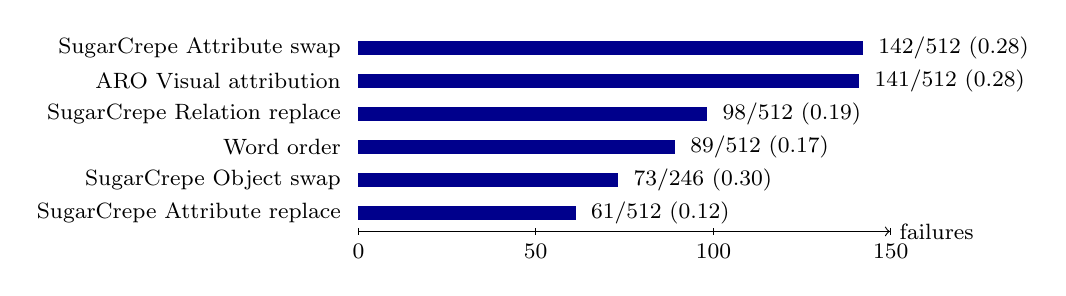
\begin{tikzpicture}[font=\footnotesize]
\node[anchor=east] at (-0.10,2.18) {SugarCrepe Attribute swap};
\draw[fill=blue!55!black,draw=blue!55!black] (0,2.10) rectangle (6.40,2.26);
\node[anchor=west] at (6.48,2.18) {142/512 (0.28)};
\node[anchor=east] at (-0.10,1.76) {ARO Visual attribution};
\draw[fill=blue!55!black,draw=blue!55!black] (0,1.68) rectangle (6.35,1.84);
\node[anchor=west] at (6.43,1.76) {141/512 (0.28)};
\node[anchor=east] at (-0.10,1.34) {SugarCrepe Relation replace};
\draw[fill=blue!55!black,draw=blue!55!black] (0,1.26) rectangle (4.42,1.42);
\node[anchor=west] at (4.50,1.34) {98/512 (0.19)};
\node[anchor=east] at (-0.10,0.92) {Word order};
\draw[fill=blue!55!black,draw=blue!55!black] (0,0.84) rectangle (4.01,1.00);
\node[anchor=west] at (4.09,0.92) {89/512 (0.17)};
\node[anchor=east] at (-0.10,0.50) {SugarCrepe Object swap};
\draw[fill=blue!55!black,draw=blue!55!black] (0,0.42) rectangle (3.29,0.58);
\node[anchor=west] at (3.37,0.50) {73/246 (0.30)};
\node[anchor=east] at (-0.10,0.08) {SugarCrepe Attribute replace};
\draw[fill=blue!55!black,draw=blue!55!black] (0,0.00) rectangle (2.75,0.16);
\node[anchor=west] at (2.83,0.08) {61/512 (0.12)};
\draw[->] (0,-0.15) -- (6.75,-0.15) node[right] {failures};
\draw (0.00,-0.11) -- (0.00,-0.19) node[below] {0};
\draw (2.25,-0.11) -- (2.25,-0.19) node[below] {50};
\draw (4.51,-0.11) -- (4.51,-0.19) node[below] {100};
\draw (6.76,-0.11) -- (6.76,-0.19) node[below] {150};
\end{tikzpicture}
}
    \caption{Largest remaining failure groups for the selected no-targeted, strong-anchor RRB model on the R030 diagnostic suite. The model still struggles with left/right spatial predicates, object and attribute swaps, and relation replacement cases.}
    \Description{Horizontal bar chart of remaining failure groups. The largest bars correspond to right-of and left-of spatial relations, followed by object swaps, attribute swaps, attribution, relation replacement, and word order.}
    \label{fig:failure_taxonomy}
\end{figure}

Figure~\ref{fig:failure_taxonomy} shows the largest remaining failure groups from the R030 diagnostic export for R028. Left/right spatial predicates remain difficult, and SugarCrepe object and attribute swaps still account for many errors. These failures are consistent with the external checks: RRB changes the relation-vs-preservation tradeoff, but it is not a complete spatial reasoning solution.

The margin information in the diagnostic report is also useful. The left/right failures have margins near zero, which means many examples are not confidently wrong by a large amount; they are ambiguous under the adapted similarity function. This is different from a failure where the model strongly prefers the counterfactual caption. Small margins suggest that additional supervision, better image grounding, or a more targeted residual direction constraint might move some examples. They do not by themselves show that the current model has the right abstraction.

Object and attribute swaps are a separate failure class. These are not purely spatial, and they indicate that the relation objective interacts with broader compositional binding. A method that only improves left/right predicates would not be enough. Conversely, a method that improves object and attribute swaps while losing retrieval may simply be changing the embedding geometry too broadly. The failure taxonomy therefore acts as a check on whether the residual is correcting the intended errors or merely shifting benchmark scores.

\subsection{Missing Baselines}

The available ablation suite compares RRB to OpenCLIP, a plain adapter, hard bottlenecks, generic hard negatives, no-targeted variants, no-channel residual controls, stronger anchoring, ROP, Winoground, and Flickr30k. It does not include standard PEFT baselines such as LoRA, text-only tuning, or vision-only tuning. While RRB shows stronger retention than naive residual controls in this study, its performance relative to widely used PEFT methods remains to be characterized in future work~\cite{hu2022lora}.

This missing-baseline caveat should change how the paper is read. The result is enough to support an internal method analysis: among the implemented designs, bounded multi-channel residual adaptation gives the best relation-preservation compromise. It is not enough to claim state-of-the-art adaptation. A direct PEFT comparison would need matched training data, the same guardrail metrics, seed repeats, and external retrieval checks. Without that, the paper should avoid language such as ``outperforms PEFT'' or ``dominates adapter baselines.''

The ROP follow-up is similarly bounded. Orthogonal or principal-subspace constraints are plausible preservation mechanisms, but they are close to existing null-space, gradient-projection, residual-gradient, and principal-subspace adaptation ideas~\cite{peng2025gnsp,luo2026keeplora,qiao2024pegp,wu2026psoft,lu2024vptnullspace}. R043 preserves COCO and ImageNet better than some RRB variants but fails the relation target. That makes it useful evidence about residual direction, not a replacement headline. The lack of relation gain in the ROP follow-up suggests that naive orthogonal constraints may be too restrictive for this training signal. We leave principal-subspace projection as a complementary guardrail to future work.

\subsection{Threats to Validity}

Several threats remain. First, the guardrail datasets are sampled. COCO uses a 1,000-image retrieval split and ImageNet uses 5,000 examples. These checks are large enough to catch catastrophic collapse, but they are not a full retrieval or zero-shot evaluation suite. Second, the relation suites are staged counterfactual benchmarks. They are valuable for isolating relation edits, but they may share template structure with the training signal. Third, the run history is a project campaign rather than a fully randomized hyperparameter study. Some comparisons are tightly matched, such as R028 versus R029, while others compare design families discovered over time.

Fourth, the paper evaluates embedding behavior, not downstream user tasks. Better relation sensitivity in a dual encoder may help retrieval, filtering, or ranking, but this draft does not test an end application. Fifth, the method is tied to OpenCLIP ViT-B/16 with LAION2B weights. Other backbones may have different baseline relation sensitivity and different tolerance for residual adaptation. Sixth, the external validity checks are negative or mixed. That makes the claim honest, but it also means that the method should not be presented as a broad compositional reasoning solution.

These threats do not erase the main result. They define its scope. The evidence supports a bounded statement about adding relation sensitivity through a residual interface while avoiding the worst guardrail failures in this run family. It does not support stronger claims about universal retrieval preservation, semantic channel discovery, or broad binding generalization.

\subsection{Practical Implications}

The practical lesson is to evaluate relation adaptation with guardrails from the beginning. If the project had selected only by relation accuracy, the hard bottlenecks and no-channel controls would have looked attractive. Their retrieval and zero-shot metrics show that they are poor candidates for a CLIP-compatible method. Conversely, if the project had selected only by COCO and ImageNet preservation, the generic-hard-negative run would have looked safe while failing to address the relation problem. The useful region is visible only when both sides are measured together.

For future experiments, the highest-value additions are not more small variations of the selected checkpoint. They are matched PEFT baselines, larger external retrieval checks, and validation sets whose relation edits differ from the training templates. A better residual-direction constraint is also promising, but it should be evaluated as a guardrail mechanism rather than introduced as a novelty claim before the evidence exists.

\subsection{Claim Boundary}

The supported claim is that anchored residual adaptation improves relation sensitivity while bounding, but not eliminating, retrieval and zero-shot degradation. The unsupported claims are just as important: RRB does not prove broad Winoground binding generalization, does not preserve retrieval losslessly, does not show semantic slot specialization, and does not establish orthogonal projection as a novel method.
